\chapter{FFmpeg Interactions}%
\label{cha:ffmpeg_interactions}

Cinelerra-GG uses ffmpeg for decoding and encoding media, thus there are many opportunities available to manipulate options.

\section{FFmpeg Early Probe Explanation}%
\label{sec:ffmpeg_early_probe_explanation}

When you open media, a series of libraries and codec functions are used to \textit{probe} the data, to see if it can determine the type of file format and codec parameters needed to correctly decode the file.  If ffmpeg probes early --- \texttt{Try FFMpeg first} is in effect for the button --- it will usually find some way to try to decode just about any contemporary media file.  But there are some times that the built in codecs are actually a better choice.  A lot of this may fall into the category of personal preference.  For example, some may prefer the mpeg library in the cinelerra code over the ffmpeg code because it has more decoding capability and seems to be more robust when the media is damaged.  In that case you will want the FF button to read \texttt{Try FFMpeg last} in the upper right hand corner of the main window.

So, if ffmpeg probes early, you will never get to use the built in libraries, and if you want to skip over buggy old libraries, use ffmpeg early probe enabled so that the newest code will be tried first.

When the icon is red, ffmpeg probes early is enabled and you will see it reads \textit{Currently: Try FFMpeg first} when moving over the FF button in the upper right hand corner of the screen.  When the icon is black, ffmpeg probes early is disabled so that ffmpeg probes late and it reads \textit{Currently: Try FFMpeg last}.  The initial default state of the icon is on, that is, ffmpeg probes first.  This is the original code behavior before ffmpeg code was added.  Suggestion is to leave it on except in a few special cases where it may be better to have early probes disabled.  When you mouse over the main menu ff toggle button, the text displays ffmpeg's \textit{Currently} set position and \textit{Click to} change it.
The ffmpeg early probe state is saved between sessions and is also affected by choices made in Probe Order (in another section). It is important to note that the various file indexes may need to be rebuilt if you change which codec is being used to decode the file.  There is a warning popup to remind you when you change the default ffmpeg early probe state (unless you have checked the box to no longer show you the warning).  You can easily rebuild the index for a specific media file by going to the Resources window, right mouse click on that media, and choose \texttt{Rebuild Index} from the popup choices.

Figure~\ref{fig:ff} show (1) reddish colored FF in upper right hand corner of main window indicating
that ffmpeg early probes is enabled; (2) \textit{Try FFMpeg last}  indicator message for ffmpeg early probes enabled (note that the color is different because you highlighted the icon); and (3) black colored FF indicates ffmpeg will be used last and you are changing the behavior so that Cinelerra warns you accordingly.

\begin{figure}[htpb]
    \centering
    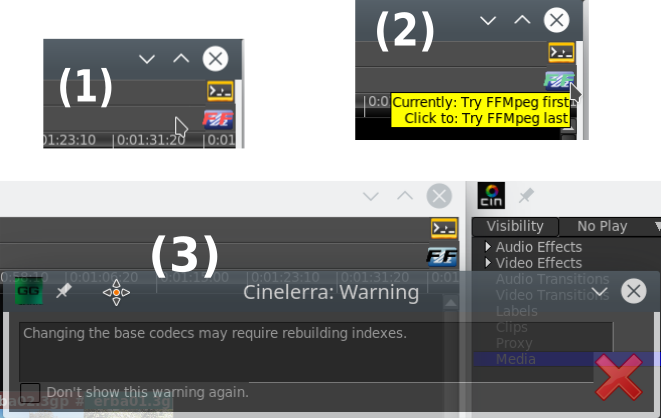
\includegraphics[width=0.7\linewidth]{images/ff.png}
    \caption{The three colors of \textit{Probe}}
    \label{fig:ff}
\end{figure}

\section{How to Create FFmpeg Options Files}%
\label{sec:create_ffmpeg_options_files}

This section describes how the FFMpeg options files work for decoding and encoding and goes into great detail.  It will make more sense if you look at cinelerra's ffmpeg config directory and the cinelerra menus at the same time.  It is meant to include everything necessary for complete understanding.  You will be able to personalize your own options files without knowing all of the information included below if you know the basics.  The word encoding is used interchangeably with the word rendering.
The possible combinations for ffmpeg options files are literally combinatorial --- that is a lot (factorial!).  The allowed media file format / codec choices are much more flexible than you might realize.  When the ffmpeg design was initially added, some parameter files which describe the choices which the program uses had to be created.  There are way too many to enumerate in the deliverable Cinelerra package.  Some quite detailed information for how ffmpeg options work is given here and hopefully, enough basics for simple understanding.  It may all seem complicated at first, but will become obvious.

\subsection{File naming convention}%
\label{sub:file_naming_convention}

In Cinelerra's ffmpeg configuration directory you will see files as listed and described below.  File type and extension names are the key for Cinelerra's use of ffmpeg.  Basically the \texttt{.opts} file extension represents options; \texttt{.dfl} represents defaults; and all the rest are media types.  For example one media type is quicktime so that \texttt{*.qt} file names would be the \textit{quicktime} choices.  In the file names below, \texttt{ext} refers to a set of files with file names matching the \texttt{*.ext} file extension.  And \texttt{typ} refers to a type of format / codec combination used, that is, the media type.

In the ffmpeg configuration directory there are a series of options files used when encoding or decoding audio or video.  They are read in the order from top to bottom and only the files needed for the current operation are added to the active configuration.

\begin{center}
    \begin{tabular}{l l}
        \toprule
        ffmpeg/ffmpeg.opts & global ffmpeg options, always used \\
        ffmpeg/decode.opts & global decoder options, used when opening existing files for decoding \\
        ffmpeg/encode.opts & global encoder options, used when creating new files for encoding \\
        ffmpeg/audio/audio.opts & audio encoder options, used when creating audio streams \\
        ffmpeg/video/video.opts & video encoder options, used when creating video streams \\
        ffmpeg/plugin.opts & parameters for ffmpeg filters as audio/video plugins \\
        \bottomrule
    \end{tabular}
\end{center}

\paragraph{Decoder options:} Normally, only \texttt{ffmpeg.opts} and \texttt{decode.opts} are used when reading/decoding files, but may be specialized if a \texttt{<path>/media.opts} exists for a given \texttt{<path>/media.ext} file.  For example, if you want to only fail on fatal errors and to always use the video filter, edgedetect, when working with your media file \texttt{dreaming.y4m}, then create a file \texttt{dreaming.opts} in the same directory with the contents of \texttt{loglevel=fatal} on the first line and \texttt{video\_filter=edgedetect} on the next.  These specialized settings will override the defaults.  The fatal loglevel is especially handy for lesser quality media.

\paragraph{Encoder Options:} Within the audio /video subdirectories of the first level ffmpeg directory, the \texttt{typ.ext} files are for encoder (rendering) setups.

\begin{center}
    \begin{longtable}{l l}
        \toprule
        ffmpeg/audio & directory of audio encoder settings \\
        \midrule
        audio.opts & options used by all audio encoders \\
        typ1.ext, typ2.ext, … & are all *.ext type choices for encoding audio \\
        ext.dfl & contains the default selection used when ext is first selected \\
        \midrule
        ffmpeg/video & directory of video encoder settings \\
        \midrule
        video.opts & options used by all video encoders \\
        typ1.ext, typ2.ext, … & are all *.ext type choices for encoding video \\
        ext.dfl & contains the default selection used when ext is first selected \\
        \midrule
        ffmpeg/format & presets needed to initialize audio / video formats \\
        \bottomrule
    \end{longtable}
\end{center}

\subsection{Option File Format / Content}%
\label{sub:option_file_format_content}

For the option files a specific format must be followed in creating the file content.
In \texttt{typ.ext} encoder parameter files, the first line is defined as:

\begin{lstlisting}[language=bash]
      muxer codec
(or) 	muxer codec | bitstream filter [ bitstream filter options ]
\end{lstlisting}

where the | represents piping the codec data through the bitstream filter. The rest of the lines in the file should look as follows:

\begin{lstlisting}[language=bash]
      # in column one is a comment
      id1   value1
(or)	id2 = value2
\end{lstlisting}

Only one equals sign is allowed and it is just for readability.  There may be any number of id / value pair lines in a media definition, including zero. A typical line might be:

\begin{lstlisting}[language=bash]
      bitrate 4000000
(or)	bitrate = 5000000
\end{lstlisting}

There are 4 special id's recognized by cinelerra which cause special processing.  They are:

\begin{description}
    \item[duration] overrides the probe duration when opening media for decoding
    \item[video\_filter] adds an video stream filter, eg. edgedetect,\dots at the stream level
    \item[audio\_filter] adds an audio stream filter, eg. echo,\dots at the stream level
    \item[loglevel] sets the library logging level, as quiet, panic, \dots verbose, debug
\end{description}

All other id's should be in the ffmpeg documentation, and correspond to the global, muxer, and codec option names and values used by ffmpeg.  For example to set the aspect ratio to 4:3, use:

\begin{lstlisting}[language=bash]
aspect 4:3
\end{lstlisting}

Below shows an example:  \texttt{decode.opts} which is used when the ffmpeg decoder is initialized.

\begin{lstlisting}[language=bash]
# apply at init decode
loglevel=fatal
formatprobesize=5000000
scan_all_pmts=1
threads=auto
\end{lstlisting}

The encoder options you see in the cinelerra menus depend on the files in these directories, \textsc{NOT THE CODE}.  If you add files, you will get to use more variety.

In the \textit{cinelerra} directory, which contains the ffmpeg configuration folder, there are the choices the program uses.  When you open an ffmpeg format popup dialog, the listbox contains all of the codec types which are identified by the file.ext extensions.  Decoding has only a few options, since the ffmpeg file probes determine most of the options by looking at the media being opened, but encoding media requires a lot of setup.  Below are some of the folders and files used to determine the configurations used by ffmpeg to decode and encode files.

These extensions create audio / video media classes:

\texttt{dvd \quad  m2ts \quad  mkv \quad  mp3 \quad  mp4 \quad  mpeg  \quad qt \quad  pro}

which become the choices in the render pulldown menu

So if you want to create a \textit{mov} codec class, add two new files to the ffmpeg configuration directory:

\texttt{audio/aud.mov}  and  \texttt{video/vid.mov}

Now you will see this as what you can choose in the rendering choices for ffmpeg.
Inside the file you will see that the first line is special.  It is the muxer and codec.  For example:

